%\section{\textit{Web Services}}
	
	\par Nos tempos atuais, com o grande fluxo de informação que percorre pela
internet, é necessário um nível muito alto de integração entre as diversas
plataformas, tecnologias e sistemas. Como uma provável solução para esse ponto,
já existem as tecnologias de sistemas distribuídos. Porém essas tecnologias
sofrem demasiadamente com o alto acoplamento de seus componentes e também com a
grande dependência de uma plataforma para que possam funcionar. Com intuito de
solucionar estes problemas e proporcionar alta transparência entre as várias
plataformas, foram criados as tecnologias \textit{web services}.
	
	
	\par De acordo com \citeonline[s.p]{erl2015}:
	\begin{citacao}
		No ano de 2000, a W3C (\textit{World Wide Web Consortium}) aceitou a submissão
		do \textit{Simple Object Access Protocol} (SOAP). Este formato de mensagem
		baseado em XML estabeleceu uma estrutura de transmissão para comunicação entre
		aplicações (ou entre serviços) via HTTP\footnote{HTTP - \textit{HyperText
		Transfer Protocol}}. Sendo uma tecnologia não amarrada a fornecedor, o SOAP
		disponibilizou uma alternativa atrativa em relação aos protocolos
		proprietários tradicionais, tais como CORBA e DCOM.
	\end{citacao}
	
	\par De acordo com \citeonline{duraes2005}, \textit{Web Service} é um
componente que tem por finalidade integrar serviços distintos. O que faz com
que ele se torne melhor que seus concorrentes é a padronização do XML
(\textit{Extensible Markup Language}) para as trocas de informações. A
aplicação consegue conversar com o servidor através do  WSDL que é o documento
que contém a estrutura do \textit{web service}.
	
	\par Segundo \citeonline{coulouris2013}, “Um serviço \textit{Web} (\textit{Web
service}) fornece uma interface de serviço que permite aos clientes interagirem
com servidores de uma maneira mais geral do que acontece com os navegadores
\textit{Web}”. Ainda de acordo com \citeonline{coulouris2013}, os clientes (que
podem ser desde um navegador até mesmo outro sistema) acessam serviços 
\textit{Web} fazendo uso de requisições e respostas formatadas em XML e sendo
transmitidos pelo uso do protocolo HTTP. O uso dessas tecnologias tende a
facilitar a comunicação entre as diversas plataformas, e atende de uma
melhor forma que as tecnologias existentes. Porém, para que haja uma
interação transparente e eficaz, entre as diversas plataformas, é necessário uma
infraestrutura um pouco mais complexa para integrar todas essas tecnologias.
Essa infraestrutura é composta pelas tecnologias já citadas e por outros
componentes essenciais para disponibilização de serviços \textit{web}, como
mostra a Figura \ref{fig:qt2}.

\begin{figure}[h!]
	\centerline{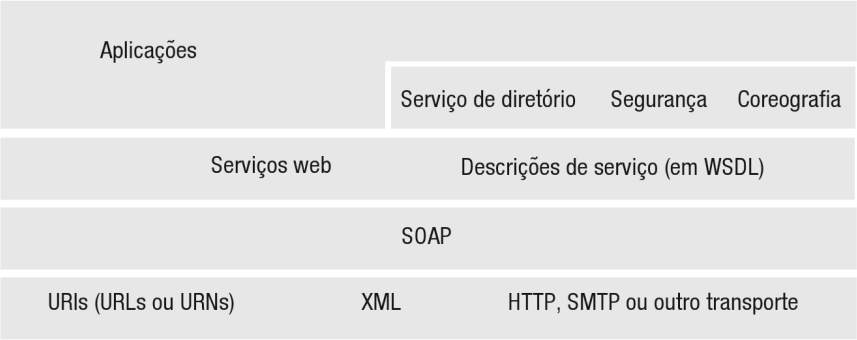
\includegraphics[scale=0.6]{./imagens/1_q_teorico/qt2.png}}
	\caption[Infraestrutura e componentes dos serviços
		\textit{web}. ]{Infraestrutura e componentes dos serviços
		\textit{web}. \textbf{Fonte:}\citeonline{coulouris2013}}
	\label{fig:qt2}
\end{figure}
	
	\par Os \textit{web services} geralmente fazem uso do protocolo SOAP, para
estruturar e encapsular as mensagens trocadas. De acordo com
\citeonline[p.381]{coulouris2013}, "o protocolo SOAP é projetado para permitir
tanto interação cliente-servidor de forma assíncrona pela Internet". Segundo
\citeonline[p.27]{sampaio2006}, "o SOAP foi criado inicialmente, para
possibilitar a invocação remota de métodos através da internet".

	\par As mensagens SOAP possuem um elemento envelope, que de acordo com
\citeonline[p.19]{saudate2013}, "é puramente um \textit{container} para os
elementos \textit{Header} e \textit{Body}". O elemento \textit{header}
transporta metadados relativos à requisição tais como autenticação, endereço de
retorno da mensagem, etc. Já o elemento \textit{body} carrega o corpo da
requisição, que nada mais é do que o nome da operação e paramêtros referentes à
mesma. É válido lembrar que todas requisições são trocadas usando SOAP, e usam
o XML como formato oficial. 
%Na Figura \ref{fig:qt3} está representado o esquema do Envelope SOAP.
	
%\begin{figure}[h!]
%	\centerline{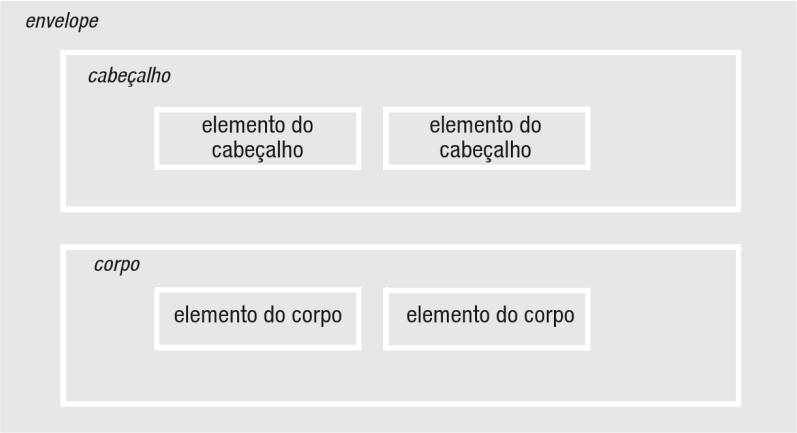
\includegraphics[scale=0.6]{./imagens/1_q_teorico/qt3.png}}
%	\caption[Esquema de envelope SOAP. ]{Esquema de envelope SOAP. 
%	 \textbf{Fonte:}\citeonline{coulouris2013}}
%	\label{fig:qt3}
%\end{figure}

	\par Os \textit{web services}, além de fornecerem uma padronização de
comunicação entre as várias tecnologias existentes, proveem transparência na
troca de informações. Isso contribui para que as novas aplicações consigam se
comunicar com aplicações mais antigas ou aplicações construídas sobre outras
plataformas.

	\par Além das tecnologias \textit{web services} tradicionais, existem os
\textit{web services} REST que também disponibilizam serviços, porém não
necessitam de encapsulamento de suas mensagens assim como os \textit{web
Services} SOAP. Este fato influencia diretamente na \textit{performance} da
aplicação, haja vista que não sendo necessário o encapsulamento da informação
requisitada ao \textit{web service}, somente é necessário o processamento e
tráfego da informação que realmente importa. As caracteristícas do padrão REST
serão abordadas na próxima seção.